\documentclass[a4paper,10pt]{article}

\usepackage[table]{xcolor}
\usepackage[ruled]{algorithm2e}
\usepackage{graphicx}
\usepackage{fullpage}
\usepackage{amsmath,boxedminipage}
\usepackage{amssymb}
\usepackage[totalwidth=166mm,totalheight=240mm]{geometry}

\parindent0mm
%\pagestyle{empty}


\usepackage{tikz}
\usetikzlibrary{arrows}
\newcommand{\bigoh}{\mathcal{O}}
\newcommand{\PP}{\mathcal{P}}
\newcommand{\avg}{\textrm{avg}}
\newcommand{\nop}[1]{}
\newcommand{\var}{\textrm{var}}
\newcommand{\E}{\textrm{E}}
\newcounter{aufgc}
\newenvironment{exercise}[1]%
{\refstepcounter{aufgc}\textbf{Exercise \arabic{aufgc}} \emph{#1}\\}
{
	
	\hrulefill\medskip}%

\renewcommand{\labelenumi}{(\alph{enumi})}

%\theoremstyle{plain}
\newtheorem{theorem}{Theorem}%[section]
\newtheorem{fact}[theorem]{Fact}
\newtheorem{lemma}[theorem]{Lemma}

%\newcommand{\solution}[1]{\bigskip \paragraph{Solution} #1}
\newcommand{\solution}[1]{}

\begin{document}

%% Header
\begin{minipage}[b]{0.58\textwidth}
	%	\centering
	\large
	School of Computer Science and Technology\\University of Science and Technology of China
\end{minipage}

\hrulefill

\vspace{0.2cm}
\begin{center}
	{\large \bf Exercise Sheet 3 for \\[1mm]
		Design and Analysis of Algorithms\\[0.5mm]
		Autumn 2022}\\
	\textcolor{red}{Due 28 Oct 2022 at 16:59}
	\bigskip


\end{center}
\vspace{0.1cm}



\hrulefill\medskip
%% Enter here the exercises !!


\newcommand{\Alg}{\ensuremath{\mathcal{A}}}



\begin{exercise}{30}

	Consider the algorithm \textsc{AnotherGreedyVC} given in Lecture 8 for the minimum vertex cover problem. Use the following example to show that the approximation ratio of \textsc{AnotherGreedyVC} is $\omega_n(1)$, where $n$ is the number of vertices in the input graph.

	\begin{center}
		\vspace{-0.5em}	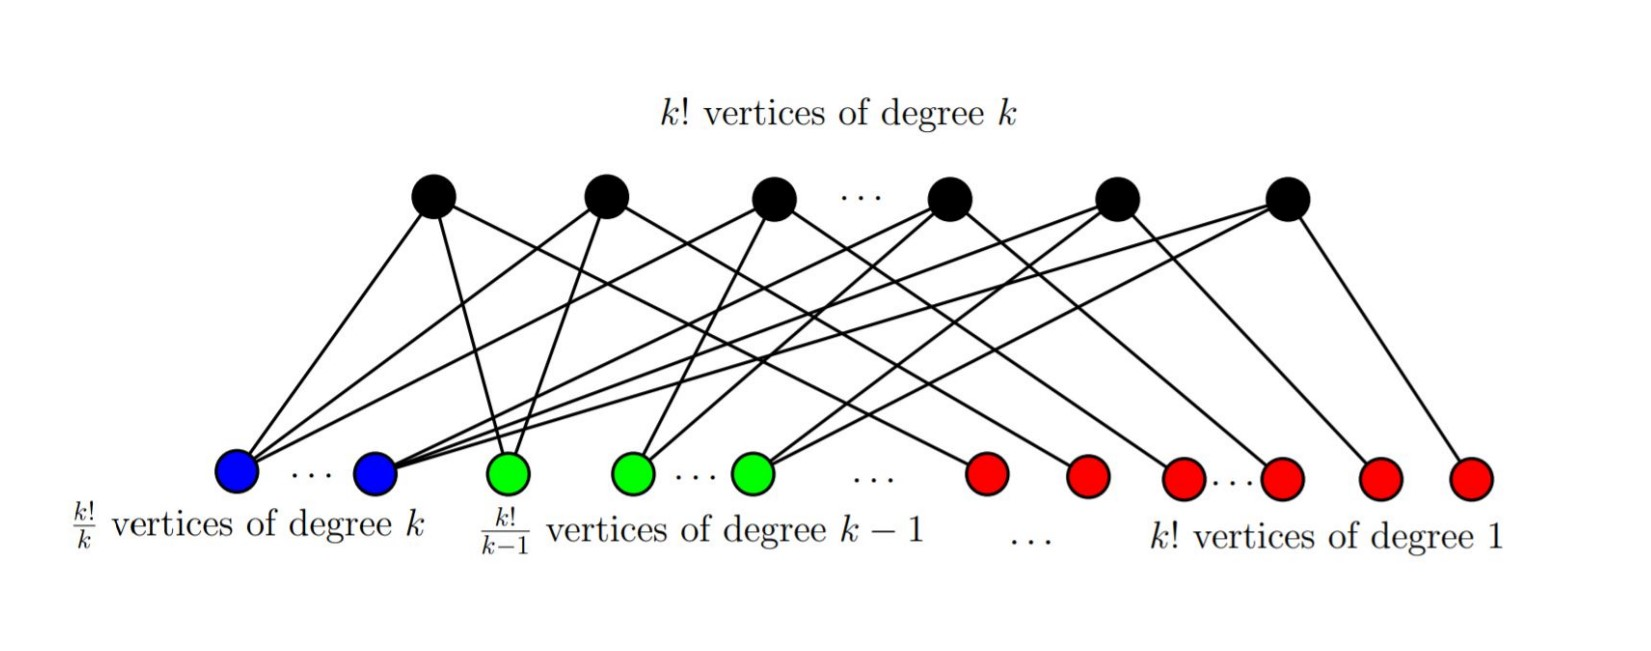
\includegraphics[width=10cm]{images/badgreedyvc.jpg}
	\end{center}


	\textbf{Solution:}
	\begin{itemize}
		\item According to the given example, $OPT=k!$ which contains all black vertices.
		\item The worst case is we choose the bottom vertices $C=k!(1+\frac{1}{2}+...+\frac{1}{k})$.
		\item $\frac{C}{OPT}=(1+\frac{1}{2}+...+\frac{1}{k})$, and the total number of vertices is $n=k!(1+1+\frac{1}{2}+...+\frac{1}{k})$
		\item Therefore, $\frac{C}{OPT}=\omega_n(1)$

	\end{itemize}




\end{exercise}



\begin{exercise}{30}

	Consider the set cover problem. Let $U$ be a set of $n$ elements. Let $\mathcal{S}=\{S_1,\dots,S_m\}$ be a collection of subsets of $U$ such that $\cup_{i=1}^m S_i=U$. Our goal is to select as few subsets as possible from $\mathcal{S}$ such that their union covers $U$.

	Consider the following algorithm \textsc{SetCover} for this problem. The algorithm takes as input $U$ and $\mathcal{S}$, and does the following:
	\begin{enumerate}
		\item Initialize $C=\emptyset$.
		\item While $U$ contains elements not covered by $C$:
		      \begin{enumerate}
			      \item[(i)] Find the set $S_i$ containing the greatest number of uncovered elements
			      \item[(ii)] Add $S_i$ to $C$.
		      \end{enumerate}
	\end{enumerate}

	To analyze the above algorithm, let $k=\mathrm{OPT}$ be the number of sets in the optimal solution. Let $E_0=U$ and let $E_t$ be the set of elements not yet covered after step $t$.
	\begin{enumerate}
		\item Show that $|E_{t+1}|\leq |E_t|-|E_t|/k$.

		\item Show that the algorithm \textsc{SetCover} is a $(\ln n)$-approximation algorithm for the set cover problem.
	\end{enumerate}


	\medskip
	%		
	\emph{Hint:} Show that the algorithm \textsc{SetCover} finishes within $\mathrm{OPT}\cdot \ln n$ steps.

	\textbf{Solution: }
	\begin{enumerate}
		\item According to the definition, the optimal solution sets must contains the $E_t$  when step $t$,
		      and in this time, the number of solution sets are most $k$, we can set it $k'$.
		      Therefore, there is at least one set which not yet select has the number of not covered elements is $|E_t|/k'$ \\
		      So, we can get $|E_{t+1}| \le|E_{t}|/k' \le |E_t |- |E_{t}|/k$
		\item As we proved in (a), $|E_{t+1}| \le |E_t |- |E_{t}|/k \le |E_{t-1}|(1- 1/k)^2  \le |E_{t-2}|(1- 1/k)^3 \le ... \le |E_0|(1- 1/k)^t$ \\
		      Set$|E_0|(1- 1/k)^t = n\exp^{-t/k} \le 1$, which means when the algorithm runs the $t+1$ steps, we can achieve the solution.\\
		      $n\exp^{-t/k} \le 1$, $n \le \exp^{t/k}$, $lnn \le t/k$, $t \ge klnn$. Therefore, the algorithm \textsc{SetCover} is a $(\ln n)$-approximation algorithm for the set cover problem.

	\end{enumerate}


\end{exercise}

\begin{exercise}{40}
	Consider the max cut problem. Given an undirected $n$-vertex graph $G =(V,E)$ with positive integer edge weights $w_e$ for each $e\in E$, find a vertex partition $(A,\bar{A})$ such that the total weight of edges crossing the cut is maximized, where $\bar{A}=V\setminus A$ and the weight of $(A,\bar{A})$ is defined to be %\begin{equation*}
	$w(A,\bar{A}):=\sum_{u\in A,v\in \bar{A}} w_{uv}$.
	%\end{equation*}

	\vspace{5em}

	Consider the following algorithm \textsc{MaxCut}.
	\begin{enumerate}
		\item Start with an arbitrary partition of $V$.
		      \item\label{step2} Pick a vertex $v\in V$ such that moving it across the partition would yield a greater cut value.
		\item Repeat step (b) until no such $v$ exists.
	\end{enumerate}

	Now analyze the performance guarantee of the algorithm.
	\begin{enumerate}
		\item Suppose that the maximum edge weight is $\lceil n^{10}\rceil$. Show that the algorithm runs in polynomial time.
		\item Let $(S,\bar{S})$ be partition output by the algorithm \textsc{MaxCut}. Show that for any vertex $v\in S$, it holds that
		      \[
			      \sum_{u\in \bar{S}, (u,v)\in E} w_{u,v}\geq \frac{1}{2}\sum_{u:(u,v)\in E} w_{u,v}
		      \]
		\item Show that the algorithm is \textsc{MaxCut} is a $1/2$-approximation algorithm for the max cut problem.
	\end{enumerate}

	\medskip
	%		
	\emph{Hint:} Use the fact that $\sum_{e\in E} w_e\geq \mathrm{OPT}$, where $\mathrm{OPT}$ is the total weight of the optimal solution.


	\textbf{Solution: }
	\begin{enumerate}
		\item According to the definition, the algorithm will check at most every edge of the graph. So the complexity of the running time is $O(|E|)$
		\item According to the algorithm step (b), the weights sum of max-cut which is the output of the algorithm is not less than the weights sum of other edges ($u\in V,v \in S$), otherwise, the algorithm can continue run the step (b) and not stop.
		      Therefore, for any vertex $v\in S$, it holds that
		      \[
			      \sum_{u\in \bar{S}, (u,v)\in E} w_{u,v}\geq \frac{1}{2}\sum_{u:(u,v)\in E} w_{u,v}
		      \]
		\item As we proved in (b),
		      \[
			      \sum_{u\in \bar{S}, v\in {S}, (u,v)\in E} w_{u,v}\geq \frac{1}{2}\sum_{u\in V,  v\in {S}, (u,v)\in E} w_{u,v}
		      \]
		      If we sum over all vertices,
		      \[
			      \sum_v \sum_{u\in \bar{S}, v\in {S}, (u,v)\in E} w_{u,v}\geq \frac{1}{2}\sum_v\sum_{u\in V,  v\in {S}, (u,v)\in E} w_{u,v}
		      \]
		      The left hand side is exactly twice the value of the cut, while the right hand side (sum of degree cuts) counts every edge twice.
		      \[
			      2W_{cut} \geq \frac{1}{2}(2\times \sum_{e\in E} w_e) \ge OPT
		      \]
		      So we get $W_{cut} \geq  \frac{1}{2}OPT$.
		      The algorithm is \textsc{MaxCut} is a $1/2$-approximation algorithm for the max cut problem.

	\end{enumerate}


\end{exercise}



\end{document}

%%% Local Variables:
%%% mode: latex
%%% TeX-master: t
%%% End:
